\documentclass[aspectratio=169]{beamer}
\usetheme{default}
\setbeamertemplate{navigation symbols}{}
\usecolortheme{structure}\setbeamercolor{structure}{fg=black}
\usepackage{tikz}
\usetikzlibrary{arrows.meta, decorations.pathmorphing}

\begin{document}

\begin{frame}{Speed of light in a coaxial cable}

\centering
\begin{tikzpicture}[
    box/.style={draw, thick, rounded corners=2pt},
    cable/.style={line width=1.4pt},
    jack/.style={circle, draw, thick, fill=white, inner sep=1.6pt},
    lbl/.style={font=\small},
  ]

  % ---- Function generator ---------------------------------------------
  \draw[box] (0,0) rectangle (2.4,1.6);
  \node[lbl, above] at (1.2,1.6) {Function generator};
  % pulse symbol
  \draw[thick] (0.4,0.5) -- (0.9,0.5) -- (0.9,1.1) -- (1.3,1.1)
               -- (1.3,0.5) -- (2.0,0.5);
  \node[font=\scriptsize, below] at (1.2,0.45) {short pulse};
  \node[jack] (out) at (2.4,0.8) {};

  % ---- T-connector ----------------------------------------------------
  \fill (3.2,0.8) circle (2.5pt);
  \draw[cable] (out) -- (3.2,0.8);

  % ---- Oscilloscope ---------------------------------------------------
  \draw[box] (6,-0.8) rectangle (10.6,3.0);
  \node[lbl, above] at (8.3,3.0) {Oscilloscope};
  \node[jack] (ch1) at (6,2.0) {};
  \node[jack] (ch2) at (6,0.2) {};
  \node[font=\scriptsize, right] at (6.1,2.0) {CH1};
  \node[font=\scriptsize, right] at (6.1,0.2) {CH2};

  % screen (white, light grid)
  \draw[thick] (7.0,-0.5) rectangle (10.3,2.7);
  \draw[black!20, step=0.4, shift={(7.0,-0.5)}]
    (0,0) grid (3.3,3.2);

  % CH1 trace: pulse directly from the generator
  \draw[very thick] (7.0,1.8) -- (7.6,1.8) -- (7.6,2.35) -- (7.95,2.35)
                    -- (7.95,1.8) -- (10.3,1.8);
  % CH2 trace: same pulse, delayed by the cable
  \draw[very thick] (7.0,0.0) -- (9.1,0.0) -- (9.1,0.5) -- (9.45,0.5)
                    -- (9.45,0.0) -- (10.3,0.0);

  % delay marker
  \draw[dashed] (7.6,-0.5) -- (7.6,2.7);
  \draw[dashed] (9.1,-0.5) -- (9.1,2.7);
  \draw[{Stealth}-{Stealth}, thick] (7.6,1.05) -- (9.1,1.05)
    node[midway, fill=white, inner sep=1.5pt] {$\Delta t$};

  % ---- Cables ---------------------------------------------------------
  % short cable -> CH1
  \draw[cable] (3.2,0.8) |- (ch1);
  % long coax (coiled) -> CH2
  \draw[cable] (3.2,0.8) -- (3.2,-1.3);
  \draw[cable, decorate,
        decoration={coil, aspect=0.6, segment length=3.2mm, amplitude=4mm,
                    pre length=0.2cm, post length=0.2cm}]
    (3.2,-1.3) -- (5.3,-1.3);
  \draw[cable] (5.3,-1.3) -- (5.6,-1.3) |- (ch2);
  \node[lbl, below] at (4.25,-1.75) {long coax, length $L$};

  % ---- Formula --------------------------------------------------------
  \node[draw, thick, inner sep=6pt, font=\Large] at (12.4,1.3)
    {$v = \dfrac{L}{\Delta t}$};
  \node[font=\scriptsize] at (12.4,0.25) {(typically $v \approx \tfrac{2}{3}\,c$)};

\end{tikzpicture}

\end{frame}

\end{document}
